\section{Wie spawnt ein Gegner und wie wird er angezeigt?}

\subsection{Methodik}

\begin{figure}[H]
    \centering
    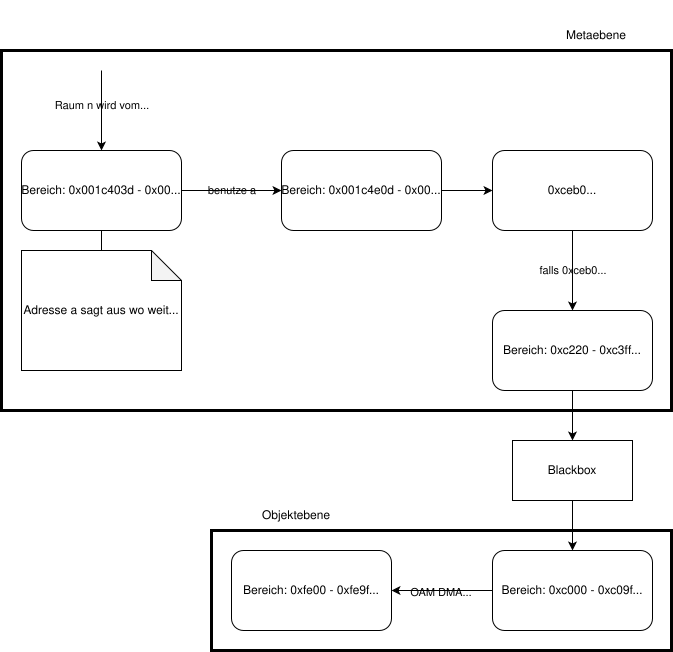
\includegraphics[width=0.8\linewidth]{Bilder/test.png}
    \caption{Übersichtsgraph}
    \label{fig:enter-label}
\end{figure}

Der vorangegangene Graph stellt eine Übersicht dar, wie ein Monster spawnt, angefangen auf einer Metaebene und endend 
auf einer Objektebene. Diesen Graphen gehen wir jetzt Schritt für Schritt durch: \\\\
Es fängt mit der Spieleraktion, mit dem Betreten des Raumes n an. Entsprechend n wird im Bereich 0x403d - 0x414c, in der 29. Rombank,
Adresse a herausgesucht. Der Bereich sieht folgendermaßen aus:
\begin{figure}[H]
    \centering
    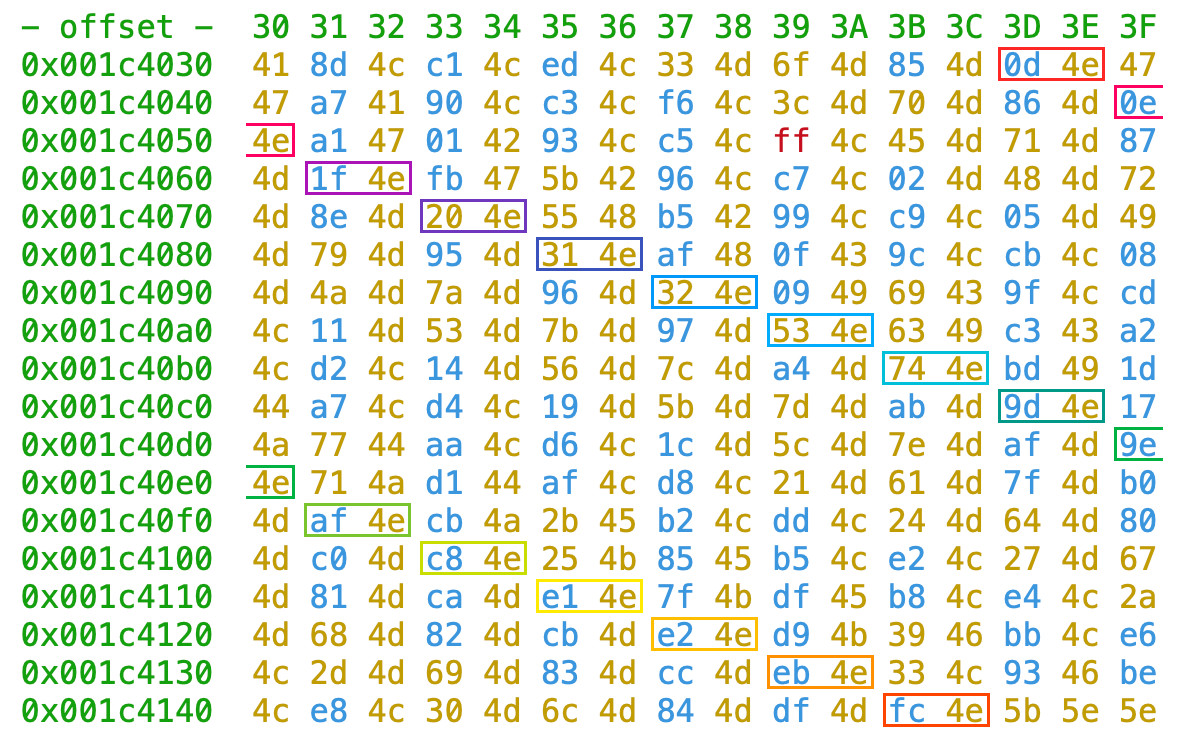
\includegraphics[width=0.8\linewidth]{Bilder/06-question03_02.png}
    \caption{Tabelle für Adresse a}
    \label{fig:enter-label}
\end{figure}

Adresse a zeigt in den Bereich 0x4e0d - 0x4efc. Der Bereich sieht folgendermaßen aus:

\begin{figure}[H]
    \centering
    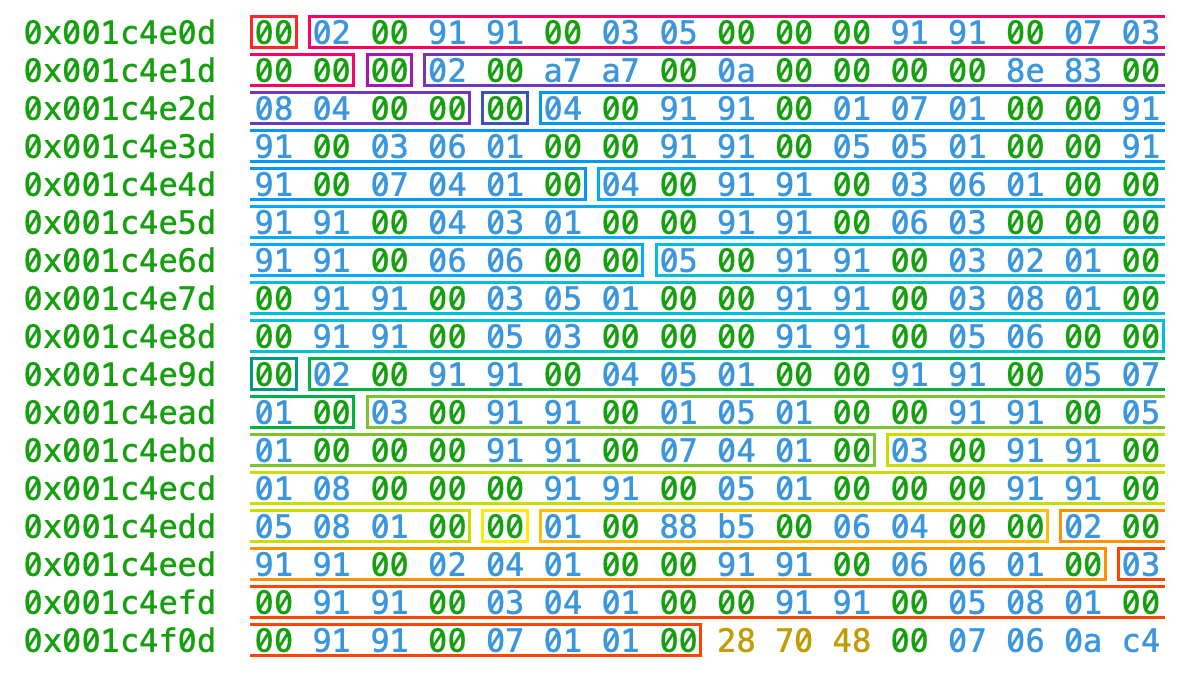
\includegraphics[width=0.8\linewidth]{Bilder/06-question03_03.png}
    \caption{Zielbereich von Adresse a}
    \label{fig:enter-label}
\end{figure}

In diesem Bereich, bzw. in jedem neu farbig markiertem Kasten, steht wie viele Monster im Raum gespawnt werden müssen und 
welche Monster gespawnt werden müssen. Am Anfang jedes neuen Bunten Kasten steht die Anzahl der zu spawnenden Monster und 
darauf folgend, in 8er Byte Paketen, die Monster Informationen. Zum Beispiel Im Raum 1 werden 0 Monster gespawnt, darauf folgend
also auch kein "Monsterpaket". Im Raum 2 werden 2 Monster gespawnt, darauf folgend 2 mal 8 Bytes.
In diesen 8er Byte Paketen steht unter anderem die Position wo das Monster spawnt. \\

In die WRAM Adresse 0xceb0 wird die Anzahl der zu spawnenden Monster hineingeschrieben. Folgende while-Bedingung wird überprüft:\\

while (0xceb0 != 0) \{ \\
\hspace*{2em} "spawne Monster"\\
\hspace*{2em} dekrementiere 0xceb0\\
\}\\

Mit "spawne Monster" ist gemeint, das 32 Bytes, die alle nötigen Logikwerte enthalten, in den Bereich 0xc240 - 0xc3ff geschrieben werden.
Diese Umgebung wird generell benutzt für Metaobjekte. Der Maulwurf selbst nimmt IMMER den Bereich 0xc220 - 0xc23f ein. \\

Die darauffolgende Blackbox sorgt dafür, dass die Gegner in Objekte mit einem Sprite übersetzt werden. Sie befindet sich zwischen der 
Metaebene und der Objektebene. Ein Metaobjekt, wie ein Gegner, wird in 4 Objekten mit jeweils einem Sprite übersetzt.\\

Die einzelnen Objektdaten werden im Shadow OAM Bereich: 0xc000 - 0xc09f vorbereitet. Ein Objekt benötigt 4 Bytes:\\
\hspace*{2em} Byte 0: Y Position\\
\hspace*{2em} Byte 1: X Position\\
\hspace*{2em} Byte 2: Tile Index\\
\hspace*{2em} Byte 3: Attributes\\

Mithilfe des OAM DMA Transfer (wird ausgeführt wenn man an die Adresse 0xff46 schreibt) werden die Daten
in den OAM Bereich kopiert. Die Objekte werden nun angezeigt.

\subsection{Ergebnis}

Wir können jetzt die Tabelle der zu spawnenden Monster verändern und somit in jedem Raum bestimmen wo und wie viele Monster spawnen.
Es gibt es Limit von insgesamt 16 Monstern, da dafür der vorgegebene Speicher nicht ausreicht.
In unserem Roomeditor können wir jetzt auch Monster platzieren.
